\subsection{Client Interface}
\label{sec:client_interface}

The client interface is illustrated in figure \ref{fig:client_interface}.
After login, the \aclient[] is greeted with the \textit{main} screen, wich gives three posebilities:
\begin{itemize}
	\item Add problem
	\item My problems
	\item Search for problem(s)
\end{itemize}

\paragraph{Add problem}as the name dictates, initiates the process of adding a specific problem to the system. Process starts by selecting what kind of problem the \aclient[] has. This is done by selecting \textit{tags} which describes the problem. Tags are grouped under categories. Each tag can only exist under one category, however if the need arises, it is possible to create a duplicate tag under another category. This does not mean that the same tag exists under two categories but two different tags with the same name exists under two different categories. We say that the problem is ``categorized'' when it has tags associated with it.
When the \aclient[] is satisfied with the categorization of his/hers problem, he/she can click ``Search'', which will make the system search for problems with similair categorization, prioritizing those with a solution attached to it.
From there, the idea is that the \aclient[] might find a problem which is identical, or almost identical, which solution will also fix the \aclient 's problem. If such a problem is found, the \aclient[] has the option to \textit{``subcribe''} to the problem, making the \aclient[] receive all the same notifications as the person who created the problem. This dramatically reduces redundancy in a case where multiple users has the same or similair problem. This also saves the \aclient s the time to create and describe a new problem in the system.
If no suitable problem is found, the \aclient[] is allowed to describe his problem with words, as well as alter the tags which he/she selected earlier, in case he/she changed his mind. Ultimately, the problem is added to the database after fully described. This process will initialize the workload monitor, for distributing the problem to a \astaff[] member, who is likely to solve the problem.
\paragraph{My problems}lists the problems created by the \aclient[], as well as the problems which the \aclient[] has subscribed to.
\paragraph{Search for problem(s)}brings the \aclient[] to the problems search-screen, where he/she can search by specifying tags which possibly are attached to the problems that the \aclient[] wiches to find.

Due to the nature of our webbased system, the \aclient[] can anytime terminate the session and logout/close.


\begin{figure}[h]
\begin{center}
 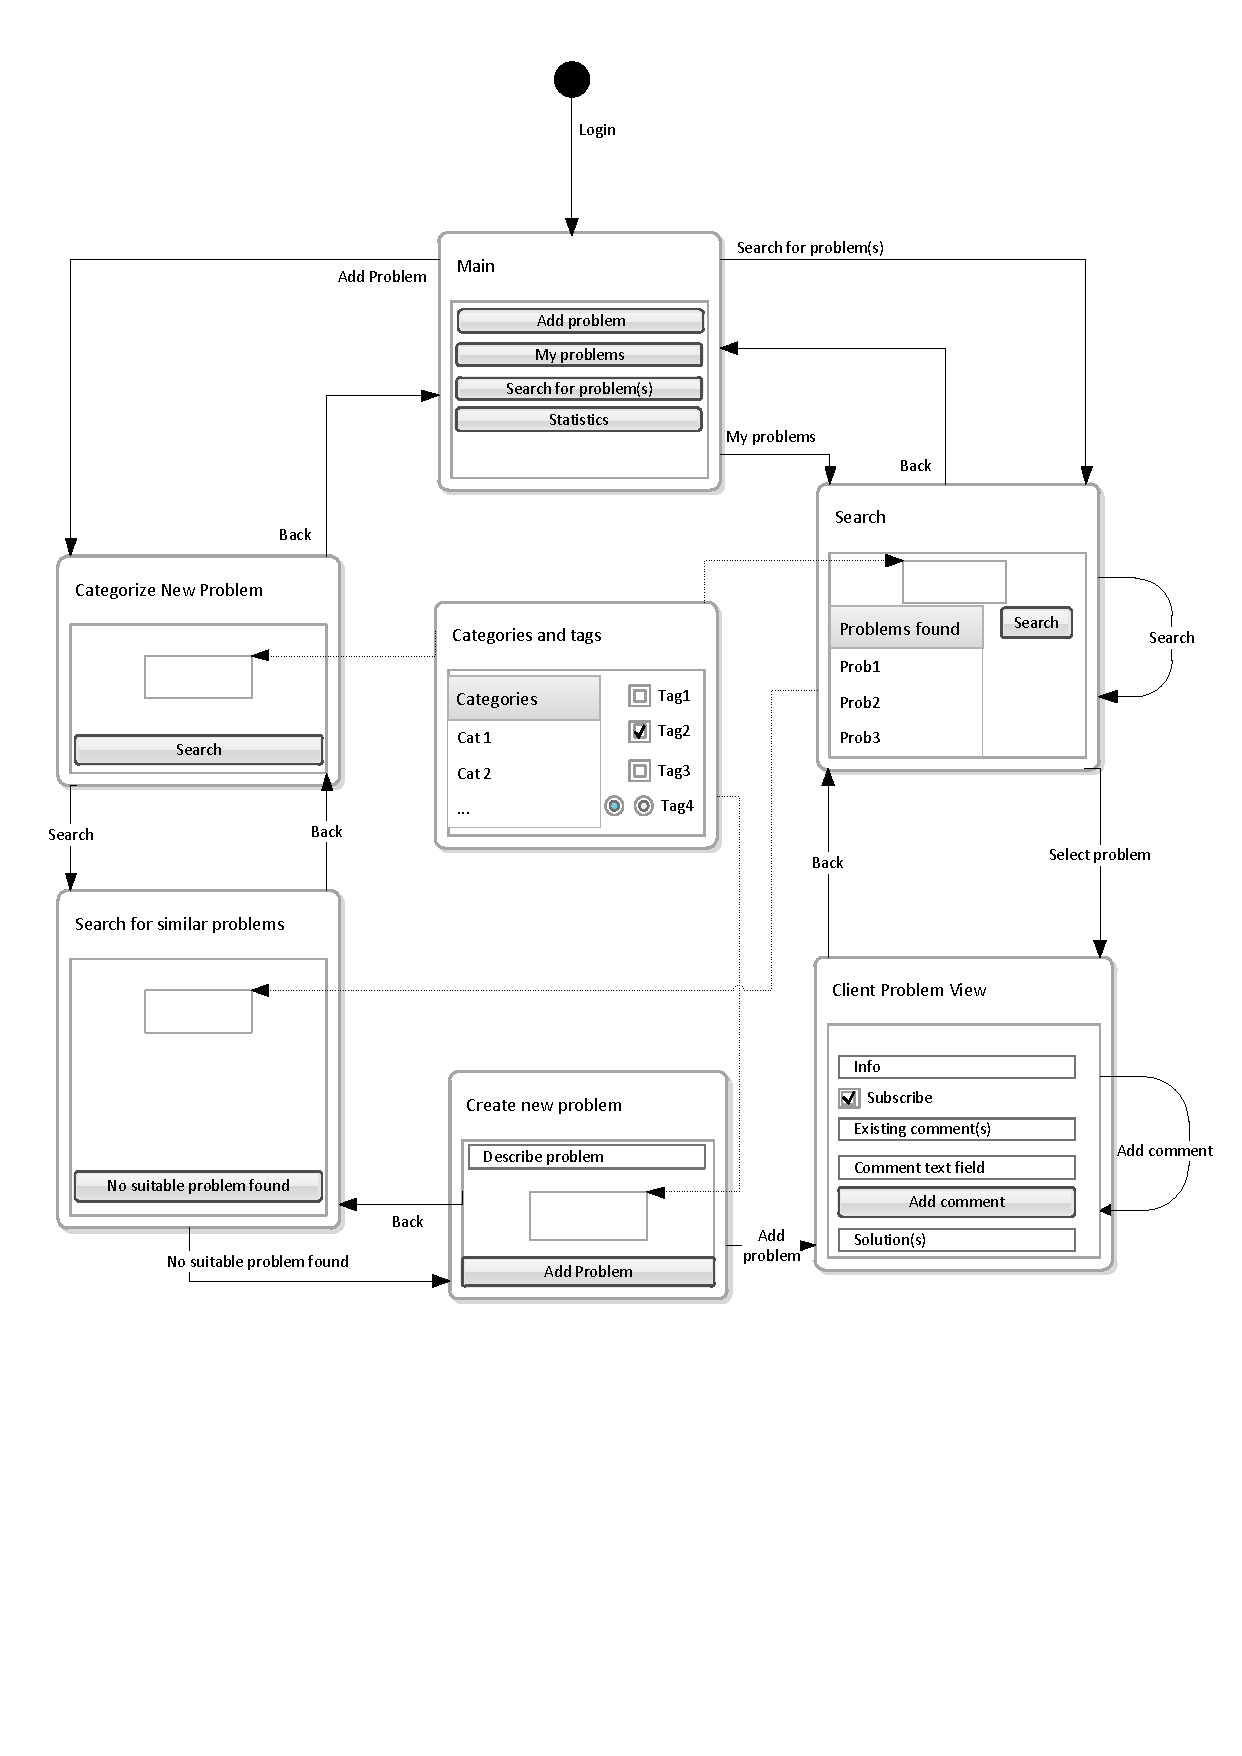
\includegraphics[scale=0.70]{input/application_domain_analysis/client_interface}
\caption{\Client[] interface}
\label{fig:client_interface}
\end{center}
\end{figure}

